\chapter{Material Layering}\label{cha:materialLayering}

	\begin{figure}
		\centering\small 
		\begin{tabular}{@{}ccc@{}}
			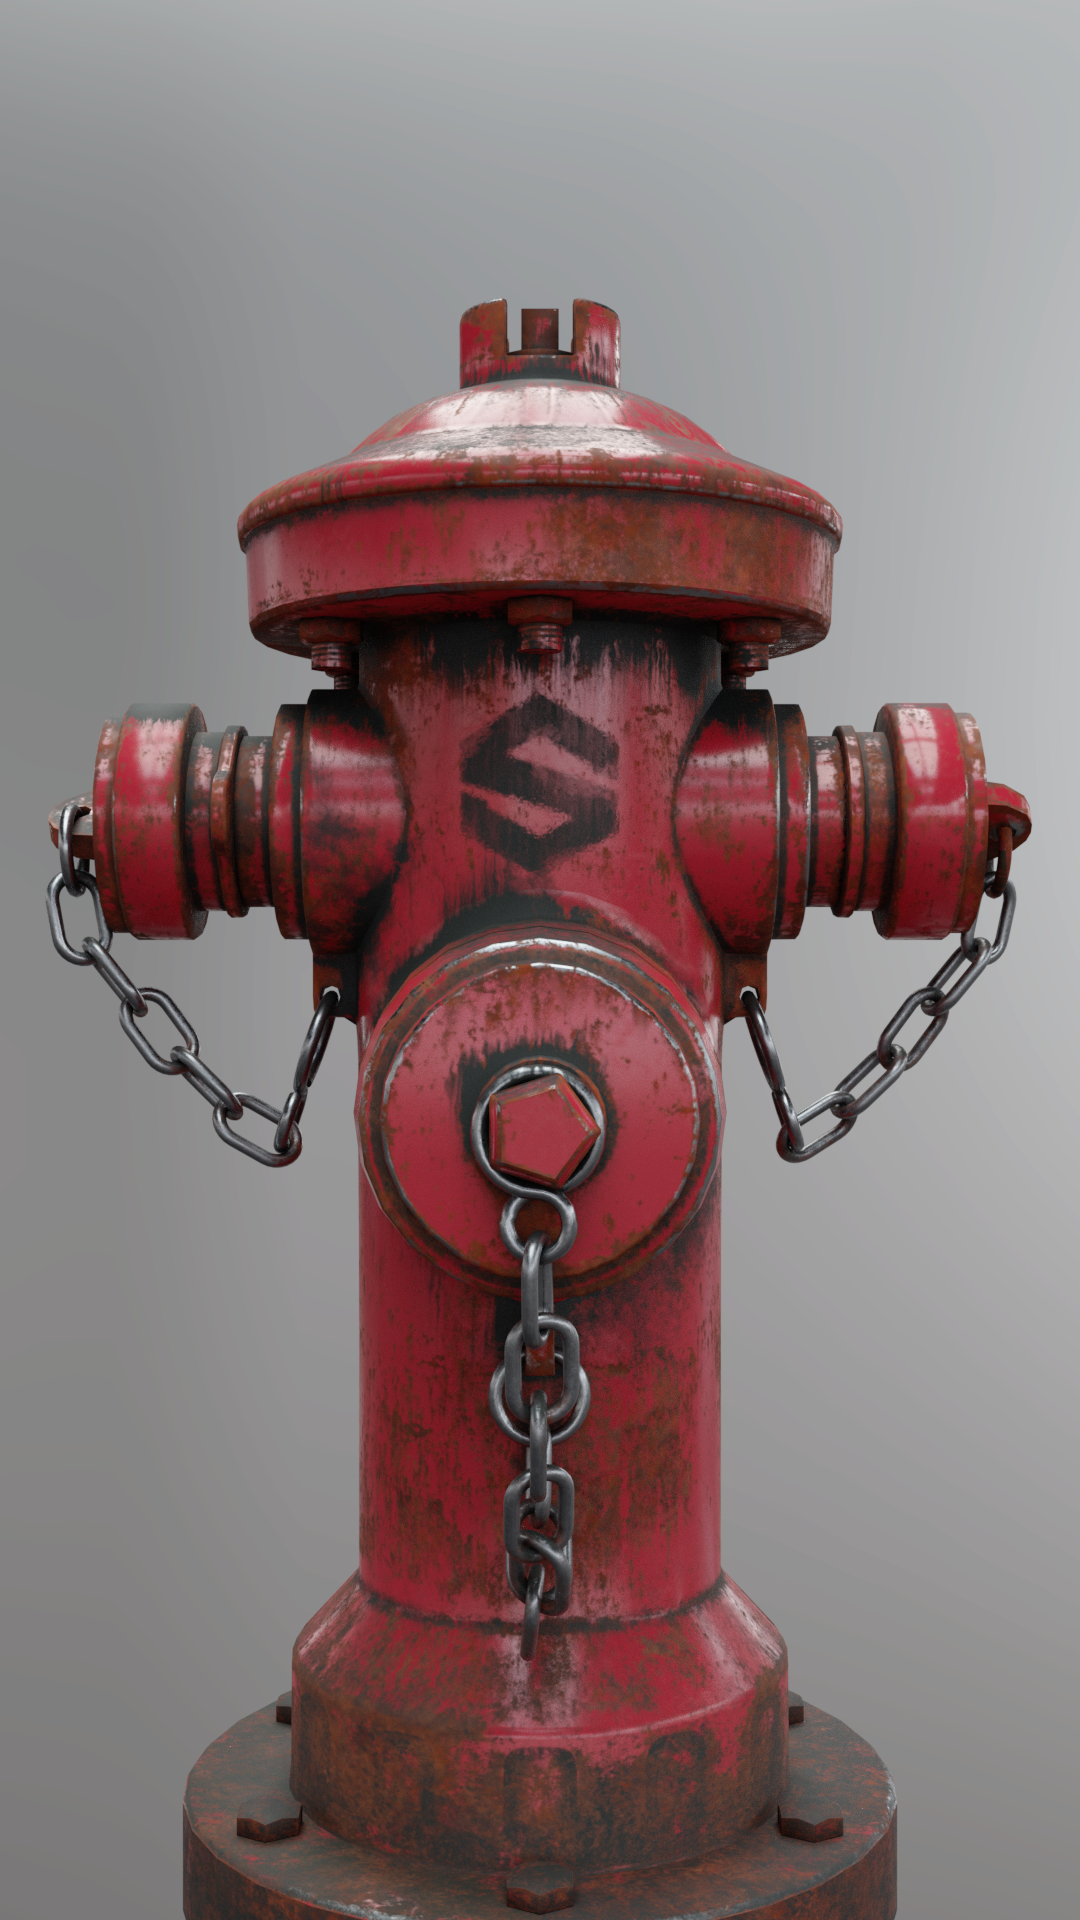
\includegraphics[width=0.3\textwidth]{images/03cha_01_04b_bxdfLayering_noNormal.jpg} &
			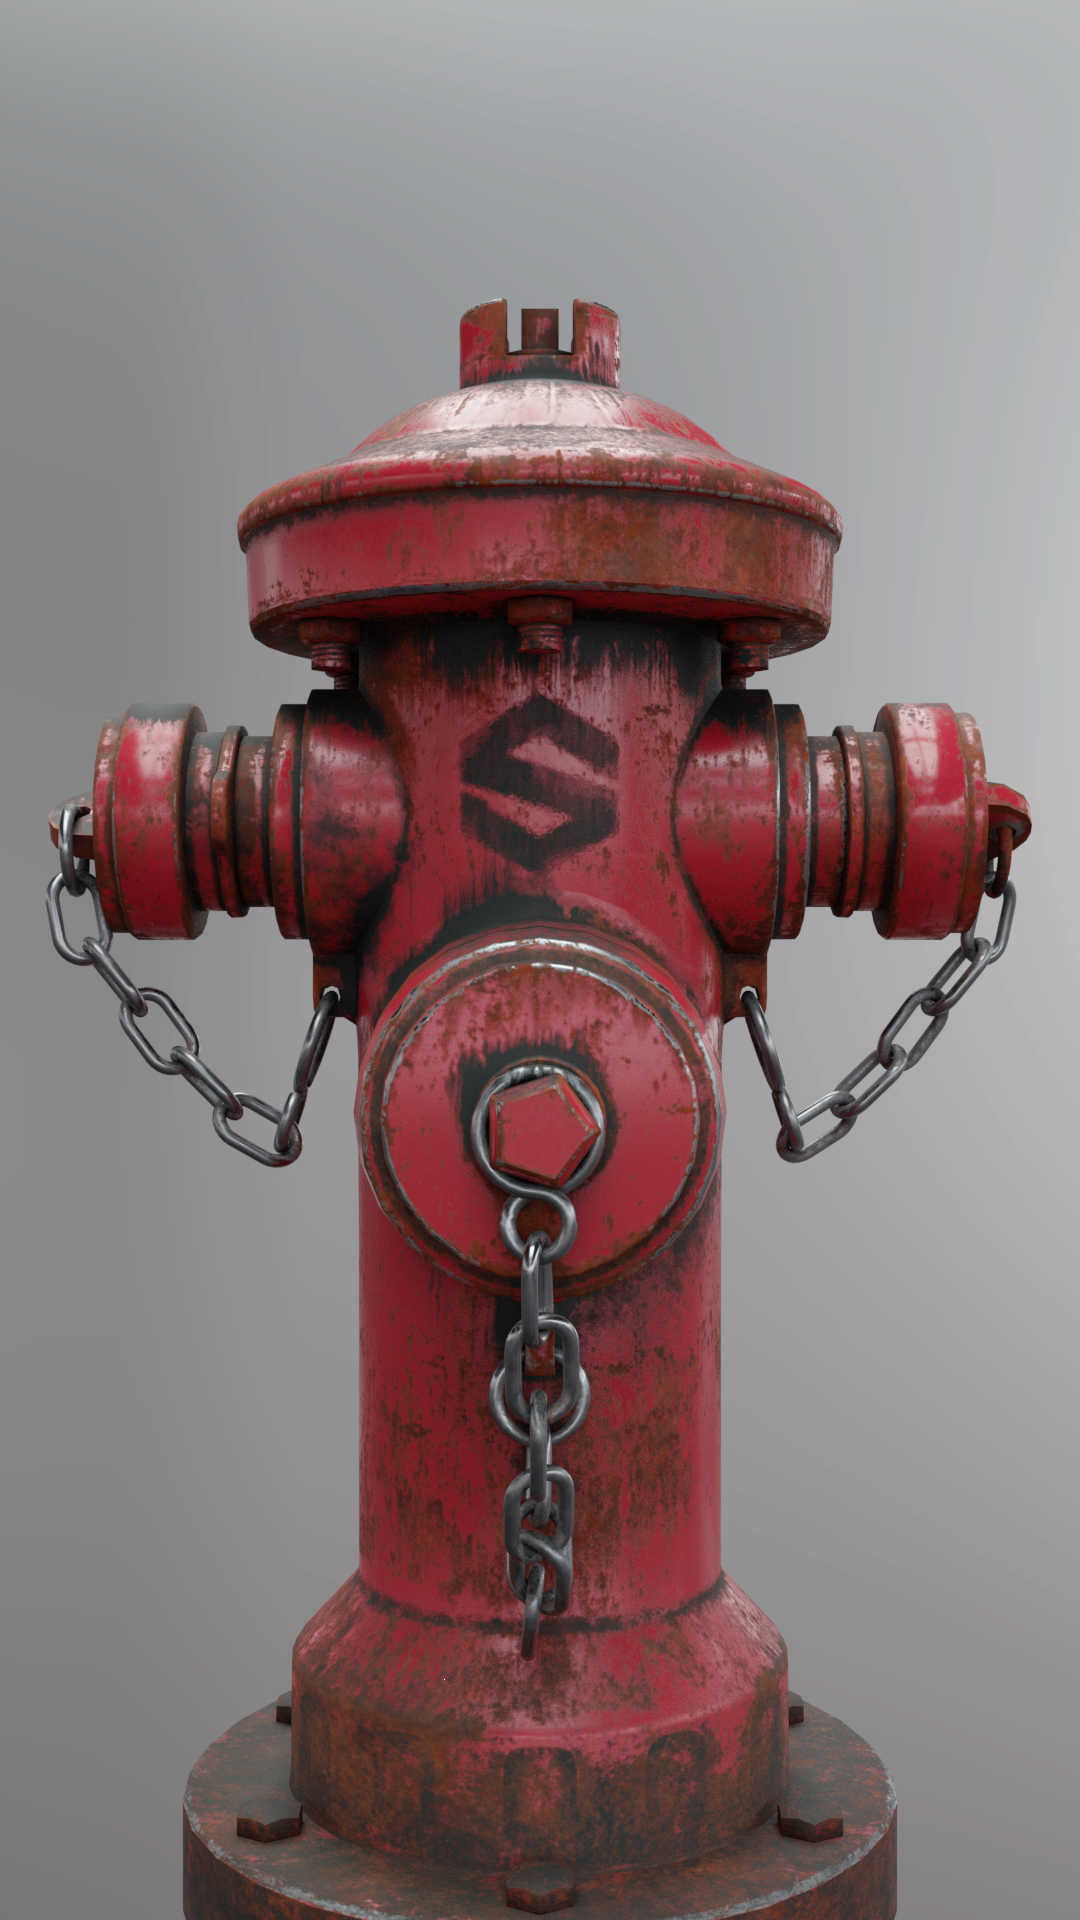
\includegraphics[width=0.3\textwidth]{images/03cha_01_04b_PatternLayering_noNormal.jpg} &
			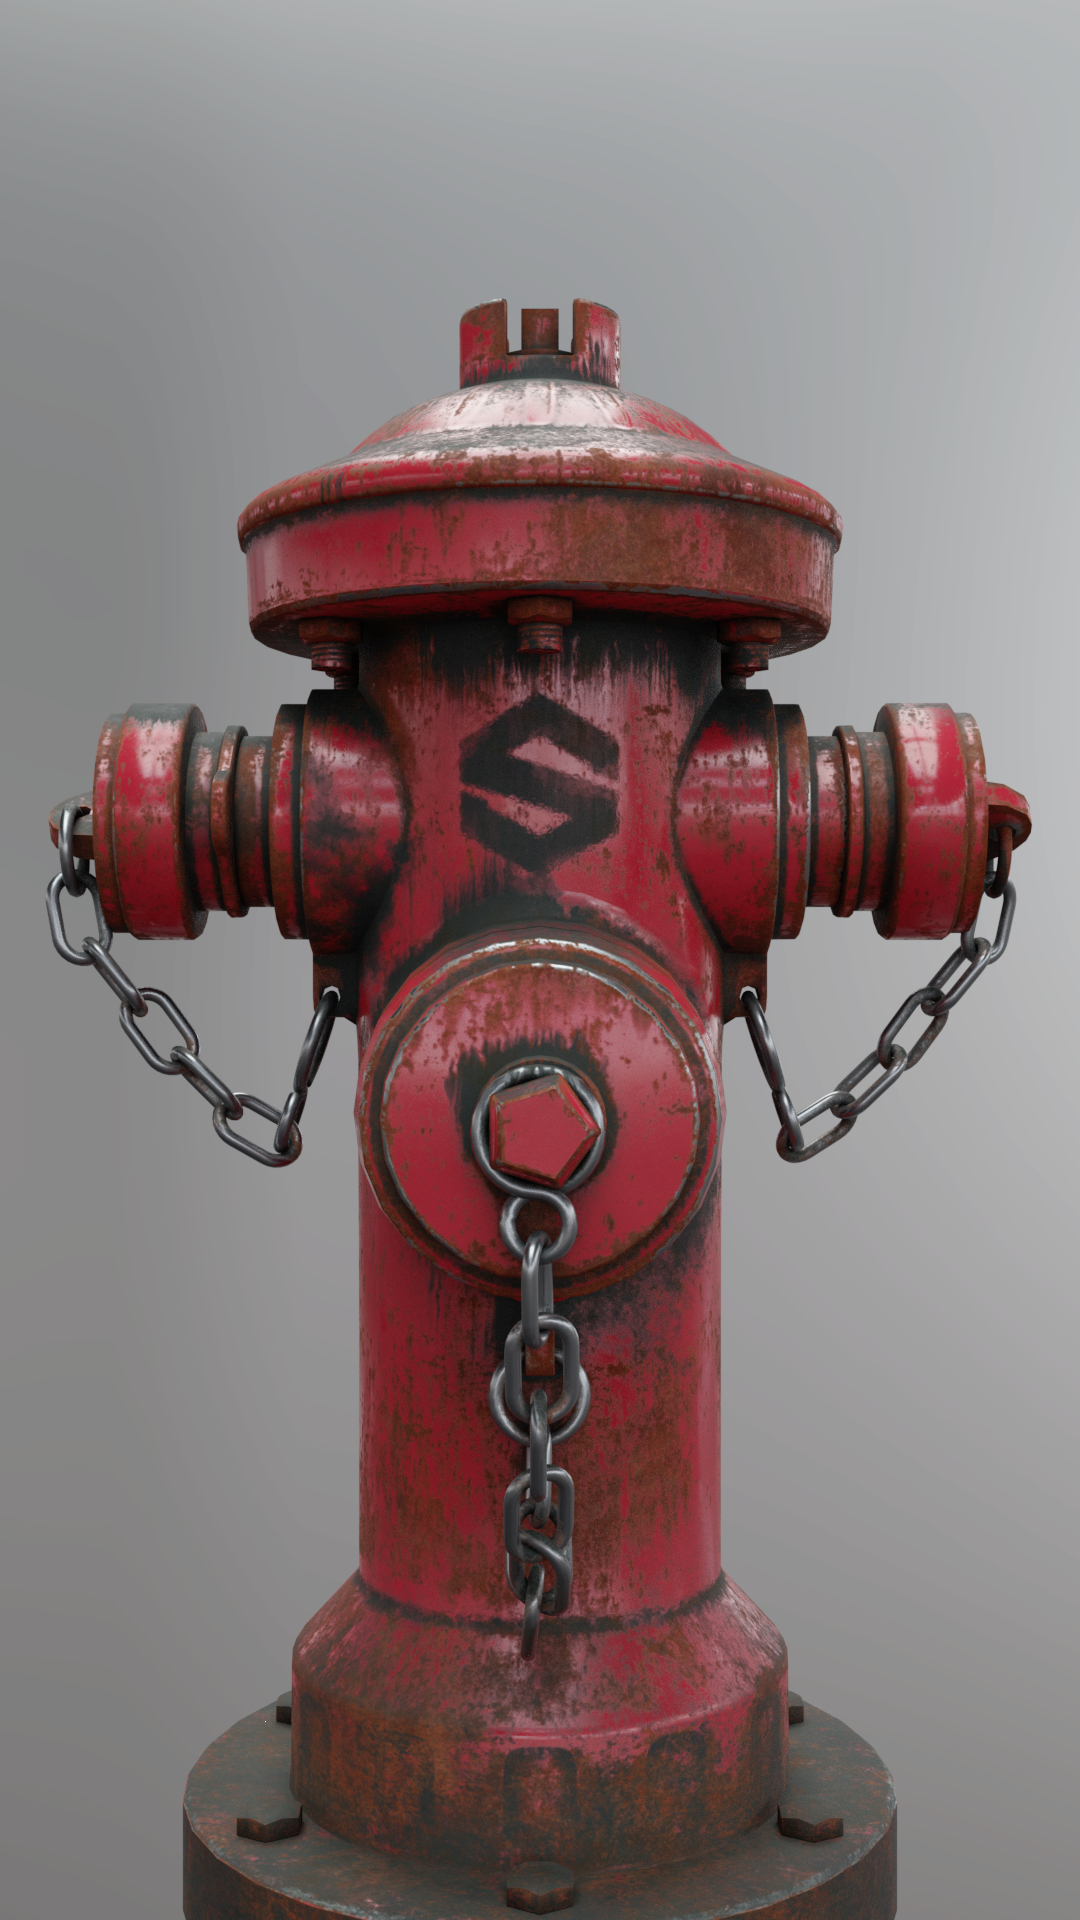
\includegraphics[width=0.3\textwidth]{images/03cha_01_04b_combined_linearInt2_noNormal.jpg} \\[6pt]
			(a) & (b) & (c) 
		\end{tabular}

		\caption{Comparison of three different shading methods. Figure (a) and (b) show different implementations of material layering: \emph{BxDF layering} and \emph{pattern layering}. Image (c) shows the reference of using traditional baked texture maps. The shading was done in \emph{Blender}, model and textures are from the \emph{Substance Share} website \cite{allegorithmic2017hydrant}.}
		\label{fig:approachesFireHydrant}
	\end{figure}


This chapter is about the current state of material layering methods. The first part provides a definition of material layering and a categorization for these methods. As the the modern game rendering pipeline is a complex system of many interlinked stages, I will try to see material layering in a larger context and not as an independent isolated component. The methods presented in this work are applied in various stages of the creation and rendering pipeline. This includes the asset creation process (e.g., modeling, texturing, normals) as well as shading and rendering (e.g., vertex shader, pixel shader, post processing).
	
Similar visual results can be achieved with different methods. An example can be found in figure \ref{fig:approachesFireHydrant}. For this example, I recreated the material setup for \emph{Allegorithmics} fire hydrant using three different methods. The images show the different material layering methods: pattern layering and BxDF layering. Both will be explained later in this chapter. The last image shows the reference image using pre-baked maps, i.e., there is a single texture for the individual material parameter inputs already containing all the information of the different base materials. The mesh and base textures used can be downloaded from the \emph{Substance Share} website \cite{allegorithmic2017hydrant}. 


\section{Definition}

This section provides a brief definition of what material layering means in the course of this thesis as well as the various methods it can be referred to in different applications and contexts. Material layering is the process of either blending distinctive base materials or recreating the physical layers of real world surfaces, illustrated in figure \ref{fig:CoatinBLending}. The former is used to create variety in different surface types; the latter is used to recreate the complex lighting effect within thin physical layers. It simulates the light scattering on, between and within physical material layers. The approaches are not directly linked to one another. Both ideas have different use cases, tools, algorithms and shaders. A distinction between the two approaches is therefore essential. 
	
	\begin{figure}
		\centering\small 
		\begin{tabular}{@{}cc@{}}
			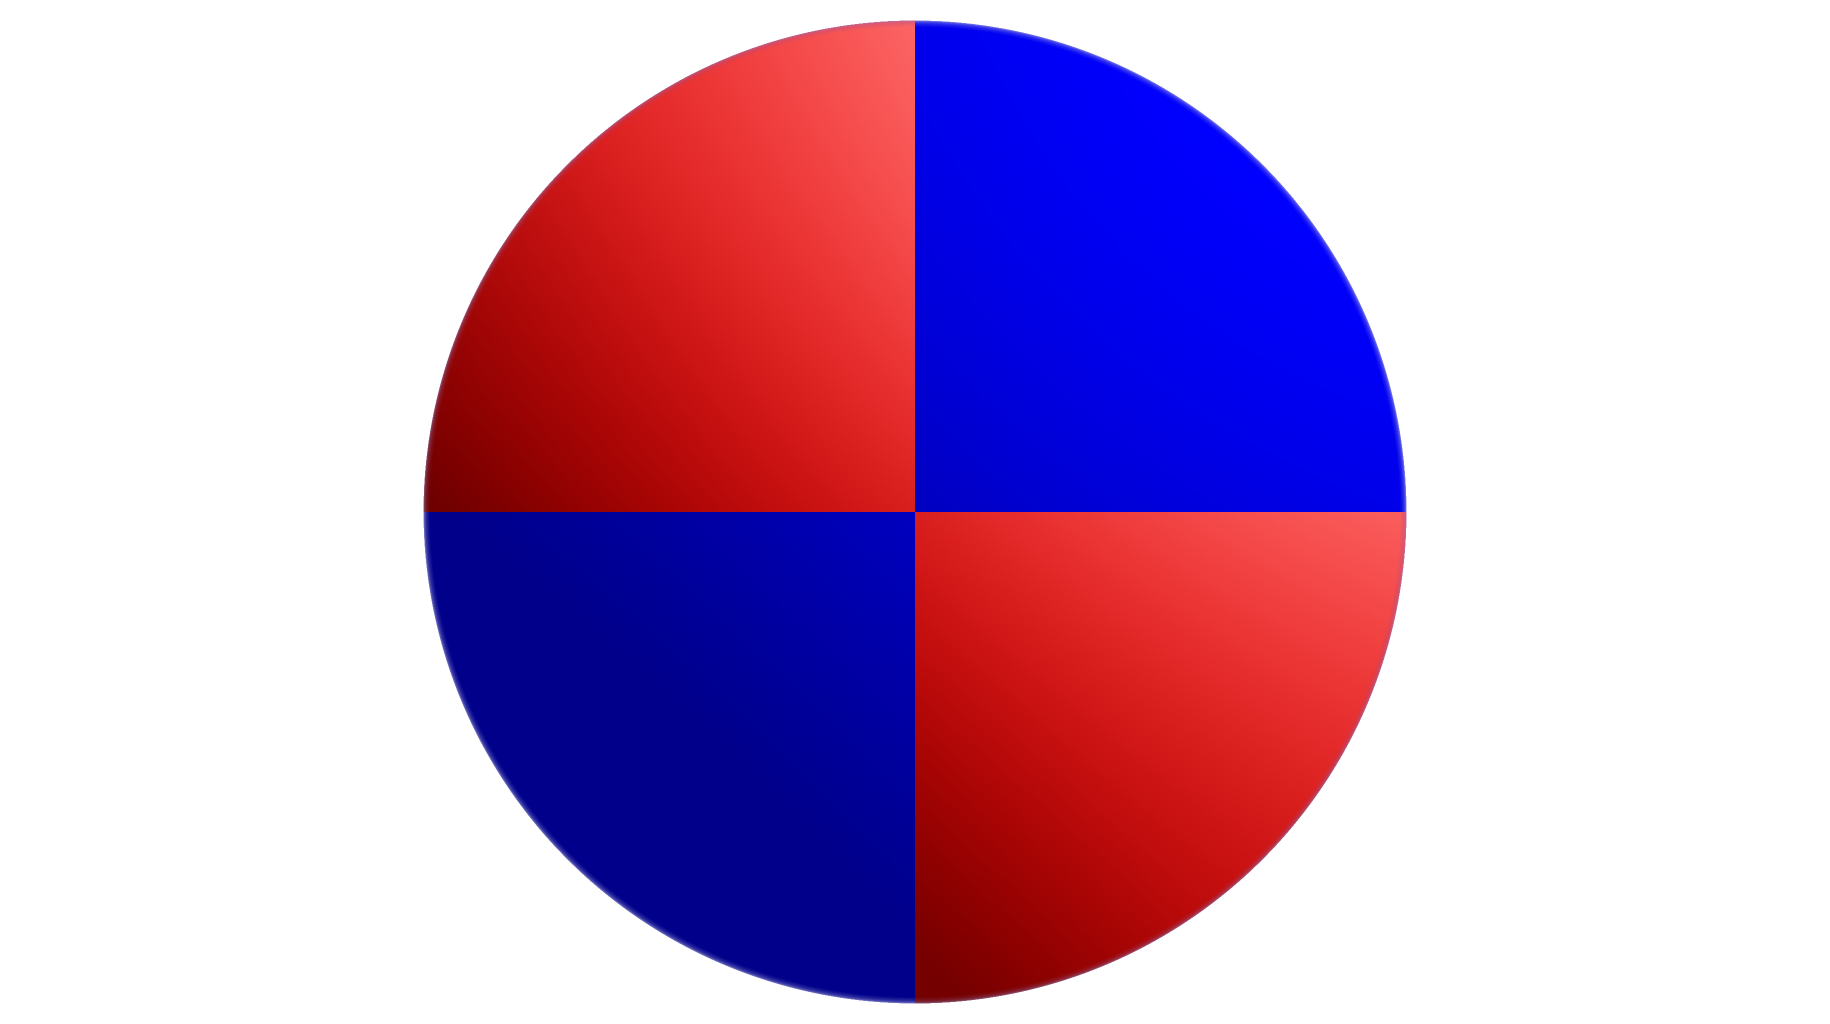
\includegraphics[width=0.475\textwidth]{images/03cha_01_masterGraphicLayering_Mat1+2.jpg} & \hfill
			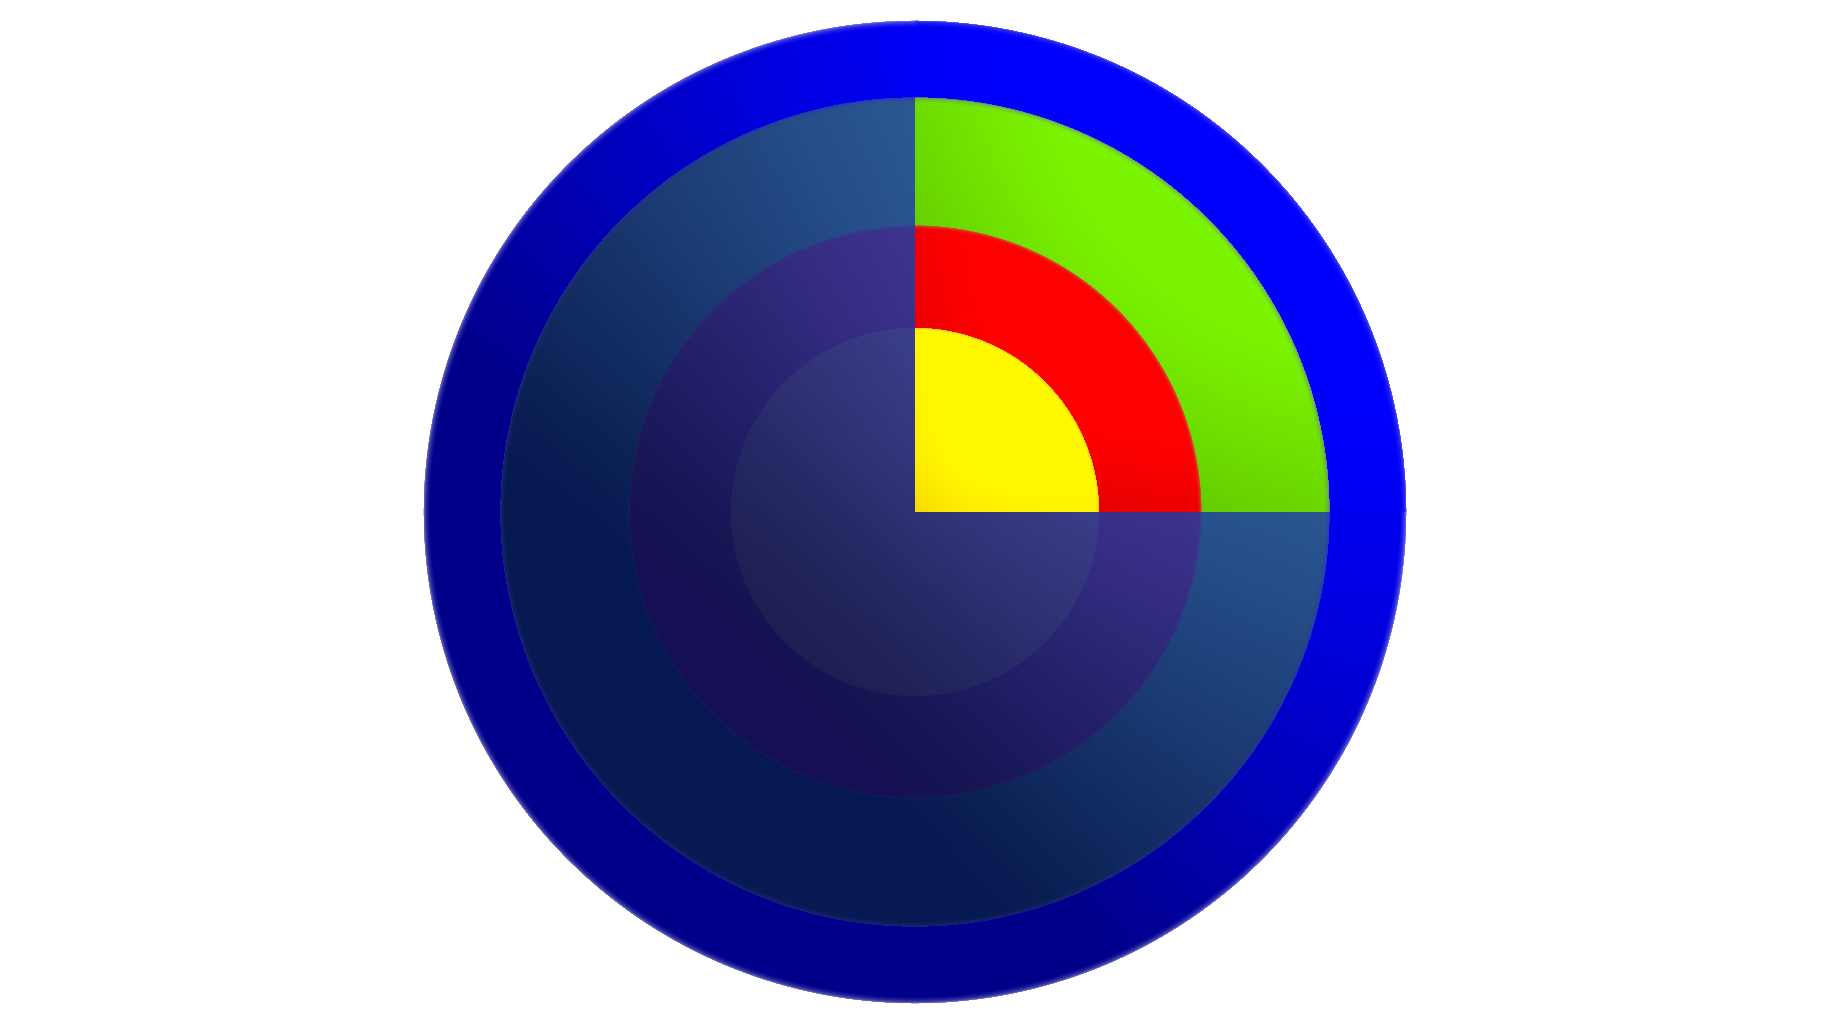
\includegraphics[width=0.475\textwidth]{images/03cha_02_masterGraphicLayering_layering.jpg} \\	
			(a) & (b)
		\end{tabular}
		\caption{{Comparison of material blending (a) and material coating (b). In material blending, masks are used to define where a base material is applied. They do not represent the physical properties of layers stacked onto one another but rather a blend defining the influence on the final output. Material coating (b) simulates an actual coating or stacking of different layers onto one another. The purpose is to recreate the complex scattering of light when passing through different layers. This is not taken into account in traditional BxDF or rasterization shading models.}}
		\label{fig:CoatinBLending}
	\end{figure}

	\begin{description}
		\item[Material Blending:]  { It describes the process of blending two distinctive base materials. This process does not take the complex process of scattering within the layers or at the layer boundaries into account.}%end new
		\item[Material Coating:] { This approach simulates the complex effects going on when stacking a---most probably translucent---layer on top of another layer. This means that the output of the first layer affects the input of the next layer. }%\end new 
	\end{description}

\section{Categorization} 

	Davide Pesare---a senior software engineer---gives  an overview of the commonly used material layering methods on his webblog \cite{pesare2017material}. He distinguishes between four different types of material layering: \emph{color layering}, \emph{pattern layering}, \emph{BxDF\footnote{The \emph{x} in \emph{BxDF} is a wildcard character and can stand for all kind of different \emph{BxDF} functions; BSDF (bidirectional scattering distribution function), BSSRDF (bidirectional scattering-surface reflectance distribution function), BRDF (bidirectional reflectance distribution function) and BTDF (bidirectional transmittance distribution function) \cite{wiki2018BxDF}.} layering}  and \emph{illumination lobe based layering}. He provides a useful guide to better understand what different approaches for layering materials exist and how they differ. 
	
	The most relevant one for this work is pattern layering as it is technically already being used for real-time applications. BxDF layering is an approach that is highly connected to ray tracing and therefore not yet applicable for the purpose or real-time applications. Nevertheless, they might become suitable for this in the future as hardware is evolving and development in real-time ray tracing is already happening as shown by a collaborative demo of \emph{Epic Games}, \emph{NVIDIA} and \emph{ILMxLAB} \cite{epic2018RealTimeRayTracing}. A paper by Belcour \cite{laurent2018efficient} has just recently been released showing an approach that makes illumination lobe based layering suitable for real-time applications. More publications and implementations in this direction might therefore follow in the next years.   

	\subsection{Color Layering}\label{sec:ColorLayering}
	
	\begin{figure}
		\centering
		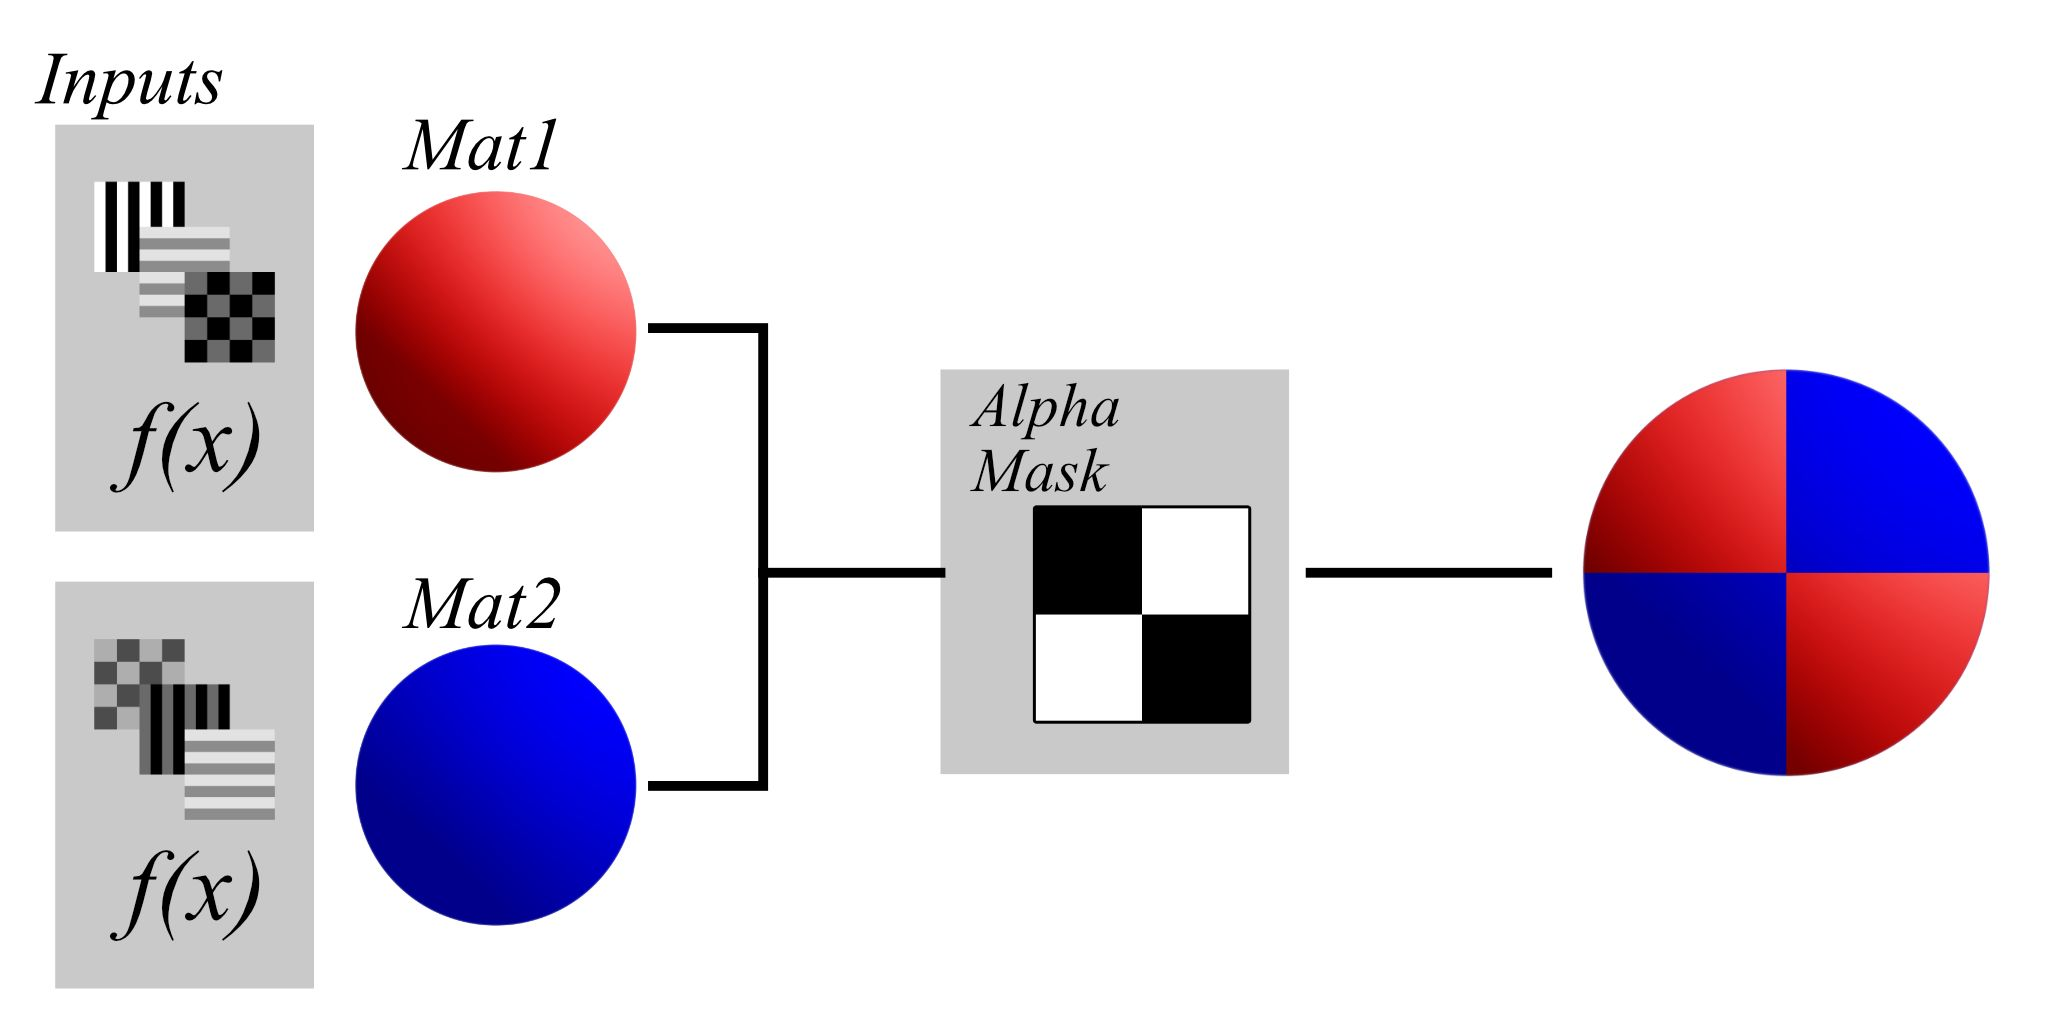
\includegraphics[width=0.75\textwidth]{images/03cha_03_ColorLayering.jpg}
		\caption[Color Layering]{
			\emph{Color layering} with two base materials. The process would look the same if applied to more base materials. Either material may have independent textures, inputs and shaders. The individual materials are computed independently from one another. Finally, the rendered output layers are blended together by using the alpha channel as a mask. If additional data like displacement is used, the blending process is more sophisticated than simple alpha blending (e.g., blending displacements properly \cite{pesare2017material}).}
		\label{fig:ColorLayering}
	\end{figure}
	
	
	 Color layering was extensively used before physically based rendering (PBR) was introduced. A set of different materials gets applied to the same object. An independent \emph{RGBA} layer is calculated for every material. These render layers contain the final object color with all illumination baked in. Finally, the different render layers for each material are blended together based on their alpha channel. Figure \ref{fig:ColorLayering} shows the schematic process of this material layering method. It can also be expanded to include advanced shading information like displacement layering \cite{pesare2017material}. Color layering results in an object being redrawn for every base material.
	

	\subsection{Pattern Layering}\label{sec:patternLayering}
		
	\begin{figure}
		\centering
		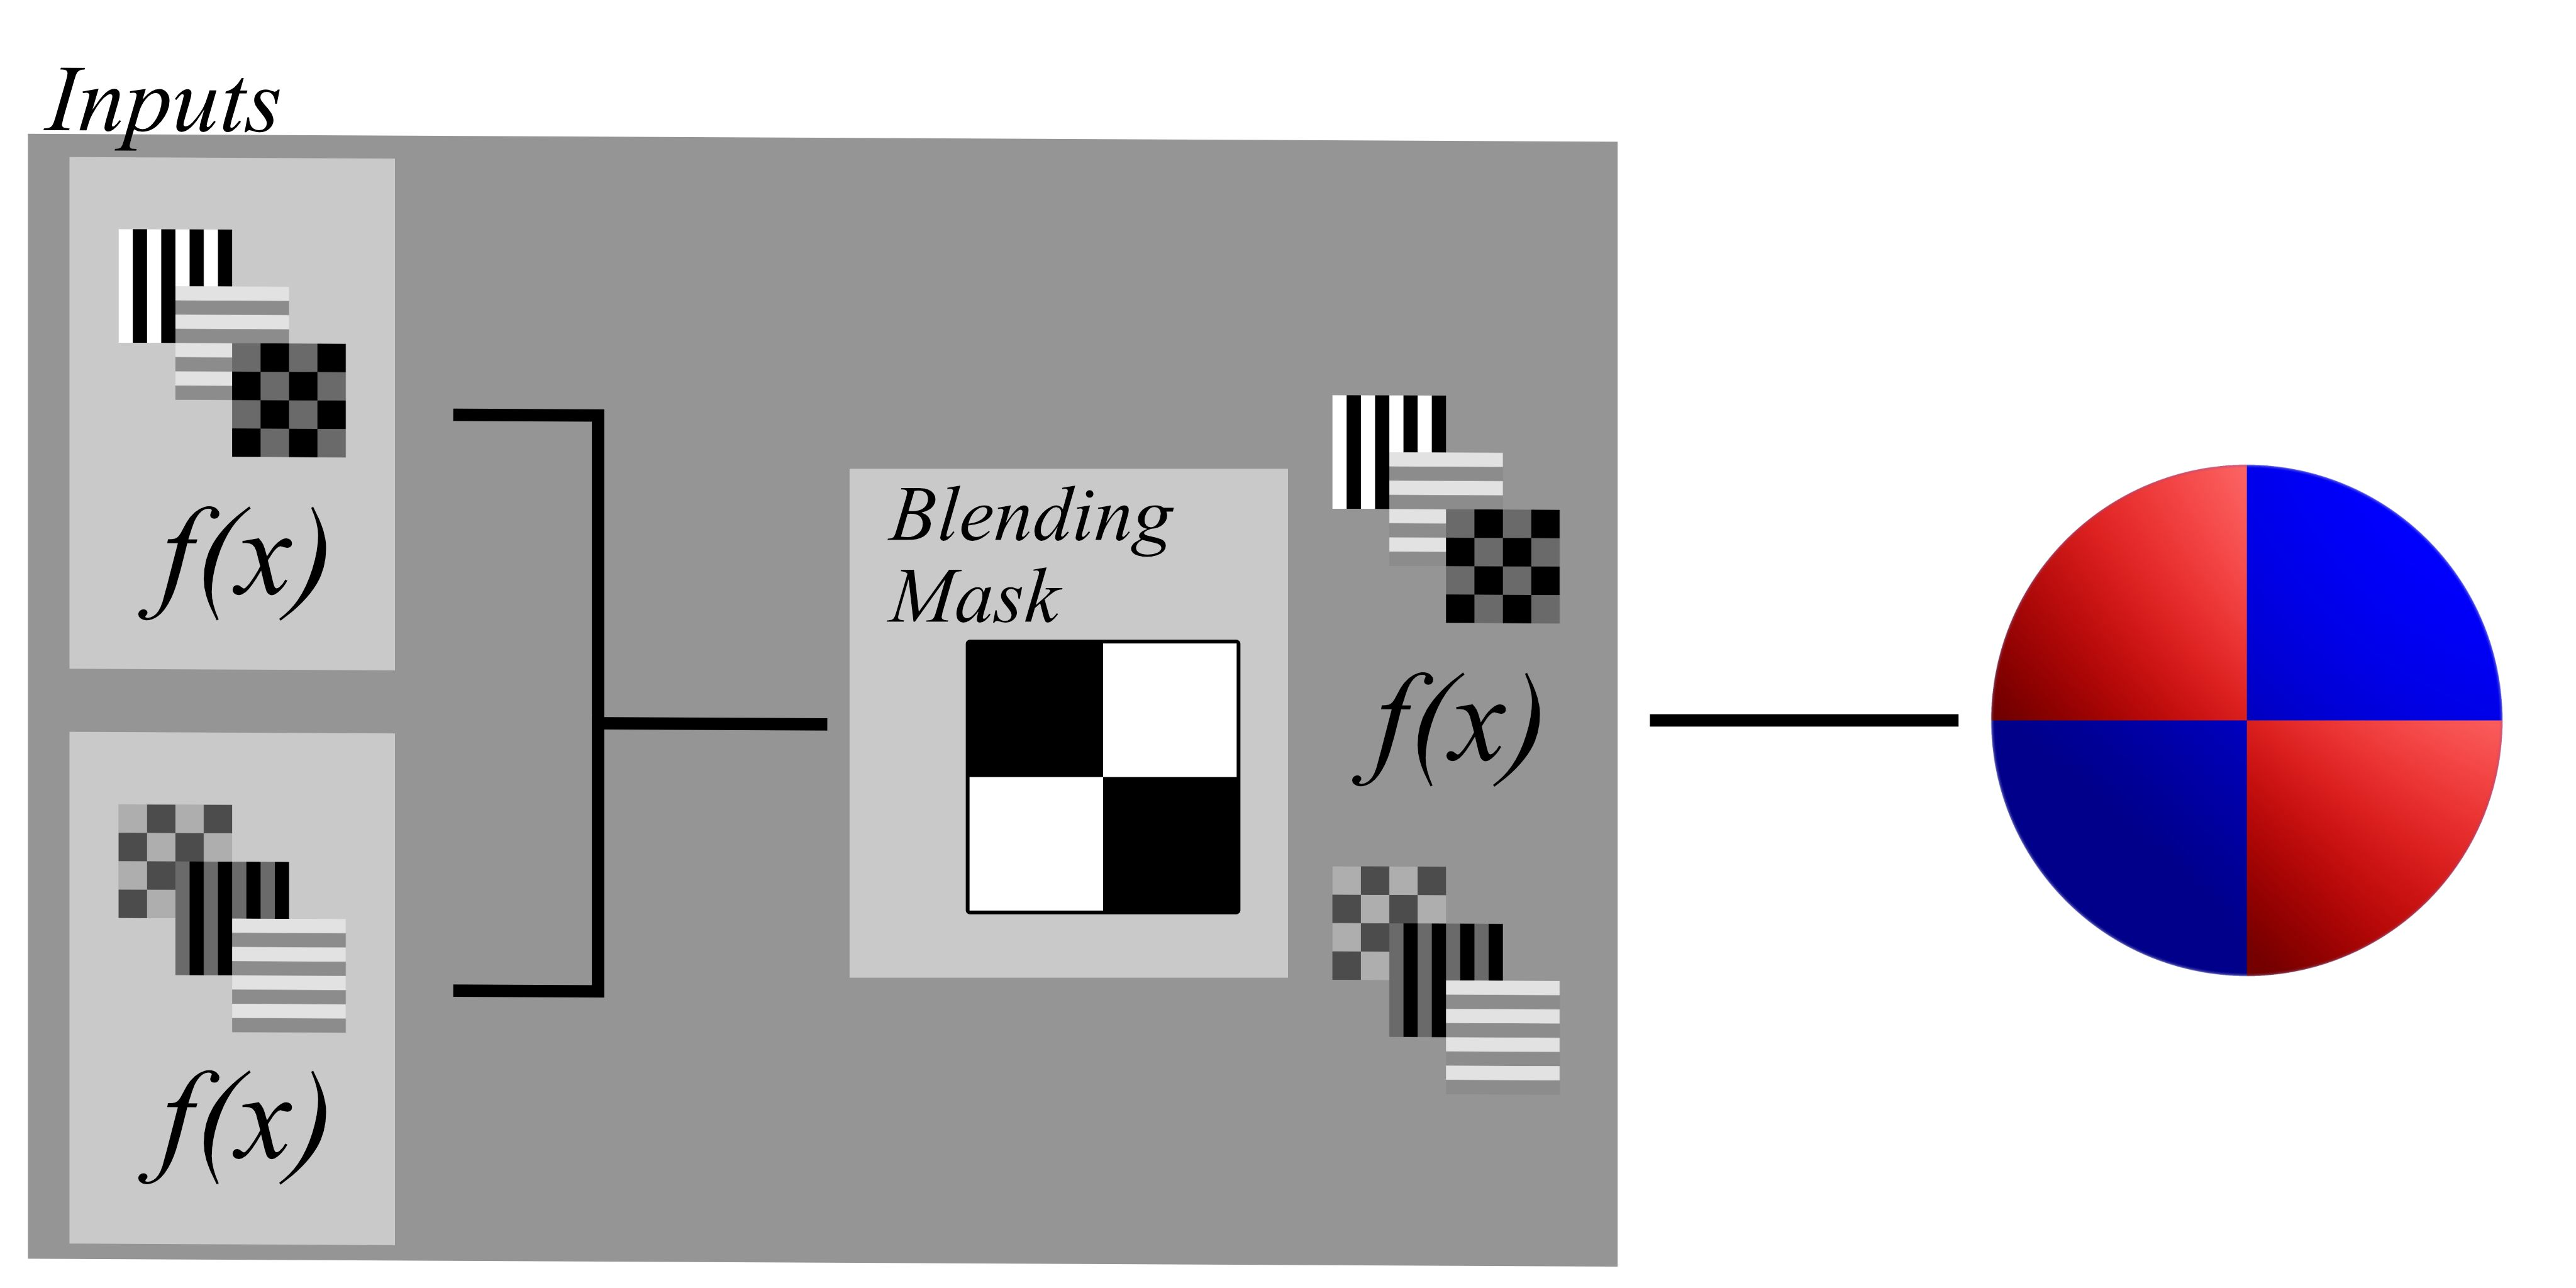
\includegraphics[width=0.75\textwidth]{images/03cha_04_patternLayering_1.jpg}
		\caption{
			\emph{Pattern layering} with two base materials. Both base material are described by independent inputs. In contrast to \emph{color layering}, the parameter inputs are blended instead of the shader outputs. A more detailed overview of how pattern layering works can be found in chapter \ref{cha:partsOfLayeredShader}.}
		\label{fig:patternLaering}
	\end{figure}
	
	The idea behind pattern layering, in contrast to color layering, is to blend the material inputs within the shader instead of their outputs. The inputs (e.g., base color, roughness, metallic) get blended with one another. Finally, the blended parameters define how the material effects the corresponding rendering pass (rasterization renderer) or illumination lobe (for a ray trace renderer). This method assumes that all base materials use the same illumination model. The inputs of the final shading programs are identical for the materials. They can therefore be packed together and send to the GPU as single job. This method reduces the material count drastically in comparison to color layering and is therefore more efficient. The features for the individual materials are limited by the shader; only inputs that are defined by the shader can be used for material layering \cite{pesare2017material}. To circumvent this issue, \emph{Epic} and \emph{The Coalition} have worked on systems that generate a shader dynamically depending on the given inputs (see section \ref{sec:matLayV2}). More detail on how \emph{UE4} and \emph{Unity} handle pattern layering and its constraints is provided in section \ref{sec:patternLayeringInUEUnity}. 

	Pattern layering is a flexible method. All kind of data types (e.g., textures, procedural noises, meshes, scene data) can be used to blend and manipulate the individual base materials. For recreating a surface that is partially covered by water, many approaches could be applied. Blending all texture maps for each and every render pass is one possibility. Another approach is to use a procedural noise that influences the roughness, base color and normal parameter inputs and creates a similar result. Pattern layering does therefore not only refer to the combining of several base materials into a layered material but also to manipulating input parameters to create a similar effect. The blending of the different parameters can be complex and therefore easily produce unintended values. Ensuring a proper blending of all inputs is the biggest challenge for a pattern based material layering system. Common issues arising form pattern layering are: a wrong roughness and index of refraction (ior) accumulation, multiple values that influence a single output and issues with blending normal vectors. These issues are further discussed in section \ref{sec:blendindIssuesLayering} on page \pageref{sec:blendindIssuesLayering}.
	

	\subsection{BxDF Layering}\label{sec:BxDFLayering}


	Bxdf layering is highly related to ray tracing. The layering system provides the renderer with the information related to which material covers which parts of the object. The blending affects the \emph{probability density functions} of the ray and is therefore independent from the individual materials themselves. The \emph{probability density function} defines the probability with which an incoming ray hits a certain material. A black mask defines the probability of $0\%$ for a ray to hit the assigned material while a white mask is equal to a probability of a $100\%$. Grey value represent a probability between a $0\%$ and a $100\%$. As shown in figure \ref{fig:BxDFLayering}, the probability for the black masked area on the left side is a $100\%$ to hit the blue \emph{MAT1}. Going further and further to the right side of the object, this probability shifts more towards the red material \emph{MAT2}. The probability increases until it is finally a $100\%$ at the white masked areas.
	
	According to Davide Pesare, the additional expanse for this approach will be minimal compared to pattern layering when the light prediction algorithms for path tracer improve \cite{pesare2017material}. In the fire hydrant example (see figure \ref{fig:approachesFireHydrant}), when comparing both methods, the rendering time for BxDF layering increased dramatically compared to pattern layering. The huge advantages of BxDF layering are: the individual materials are not limited by the constraints of a single shader, the blending is physically more accurate than pattern layering and the need for complex pipeline tools to assure the proper blending of individual lobe inputs disappears. By only influencing the probability density function the materials are completely independent from one another. This removes the technical issues for pattern layering---mentioned before---when blending different materials. Although BxDF layering is more versatile and less complex than pattern layering, it is still not able to recreate complex stacking of different materials, as explained by Andrea Weidlich et al. \cite[p.\,9]{weidlich2011thinking}:
		
	\begin{itquote}
		Materials (i.e., BRDFs) can be stacked, but only with an opacity channel; they do not influence each other. This means that a rough surface on top of a smooth surface will not increase the roughness of the underlying surface (although this would happen in reality). 
	\end{itquote} % \cite[p.\,9]{weidlich2011thinking}

	\begin{figure}
		\centering\small 
		%\begin{tabular}{@{}c@{\hspace{12mm}}c@{}} %
		\begin{tabular}{@{}cc@{}}
			\multicolumn{2}{c}{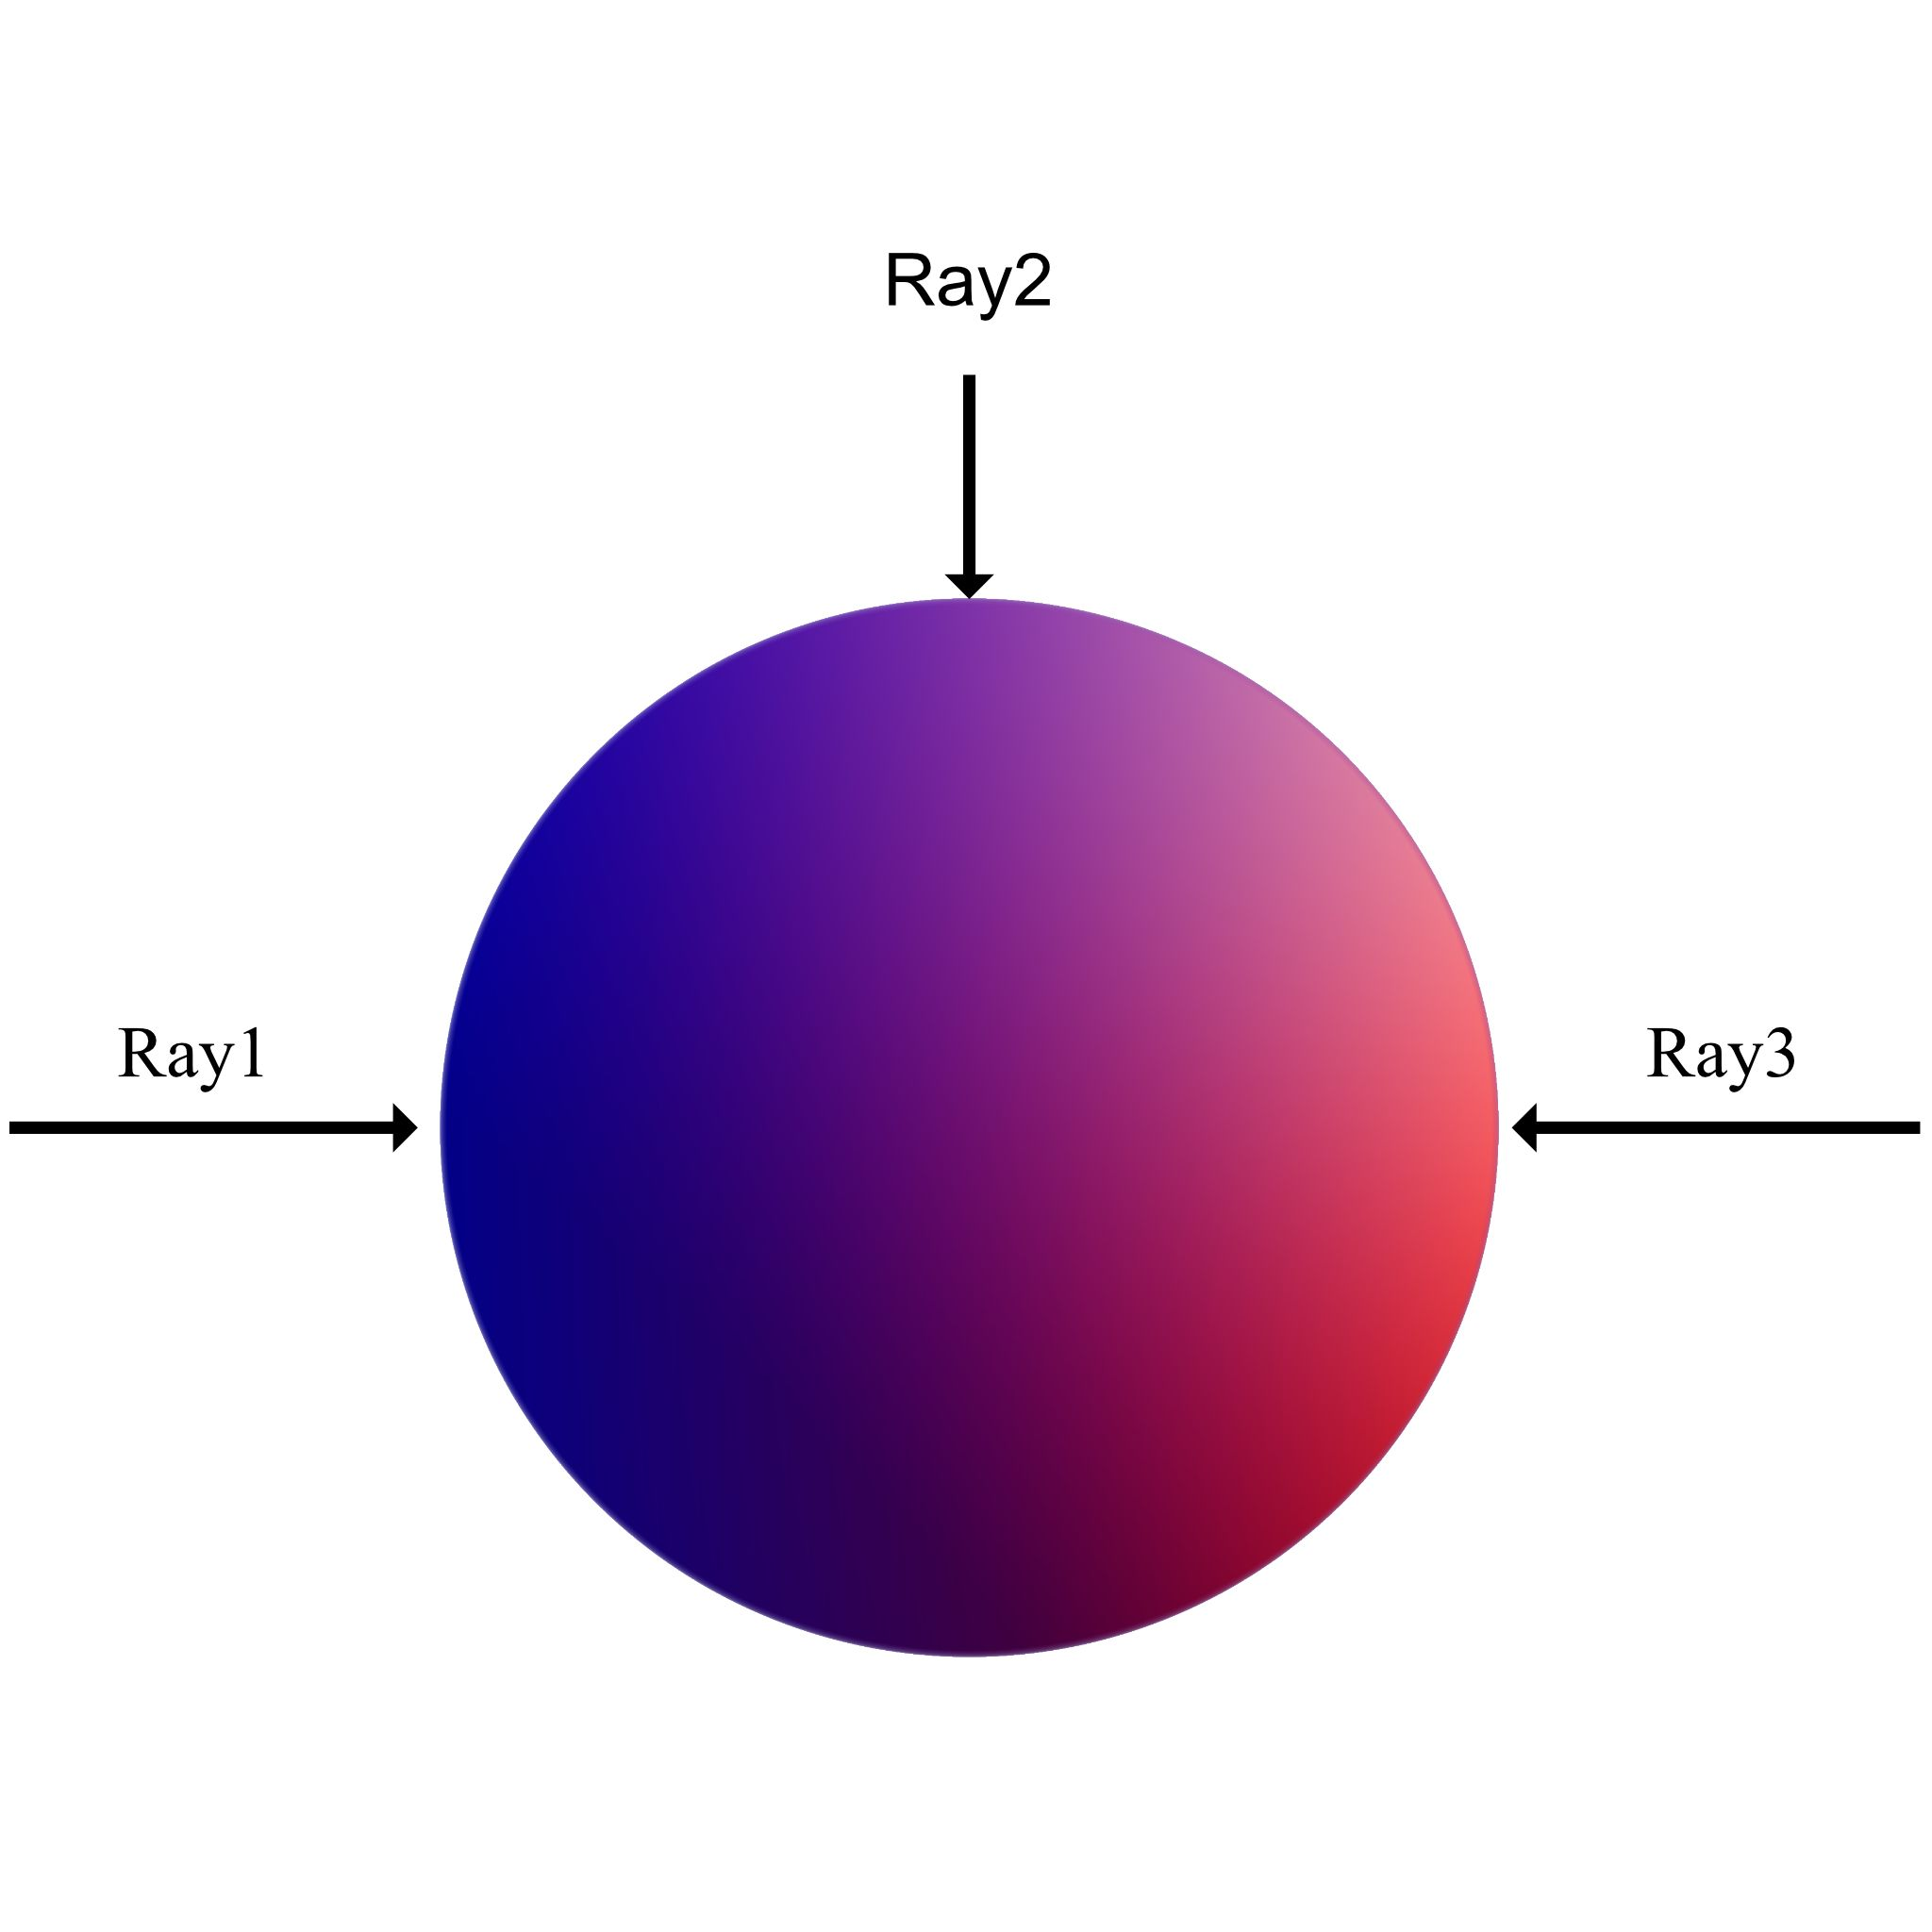
\includegraphics[width=0.5\textwidth]{images/03cha_05_bxdfLayering_1.jpg}} \\
			\multicolumn{2}{c}{(a)} \\[6pt]	%vertical extra spacing (4 points)
			
\includegraphics[width=.475\textwidth]{images/03cha_05_BxDFLayeringMask.jpg} &
			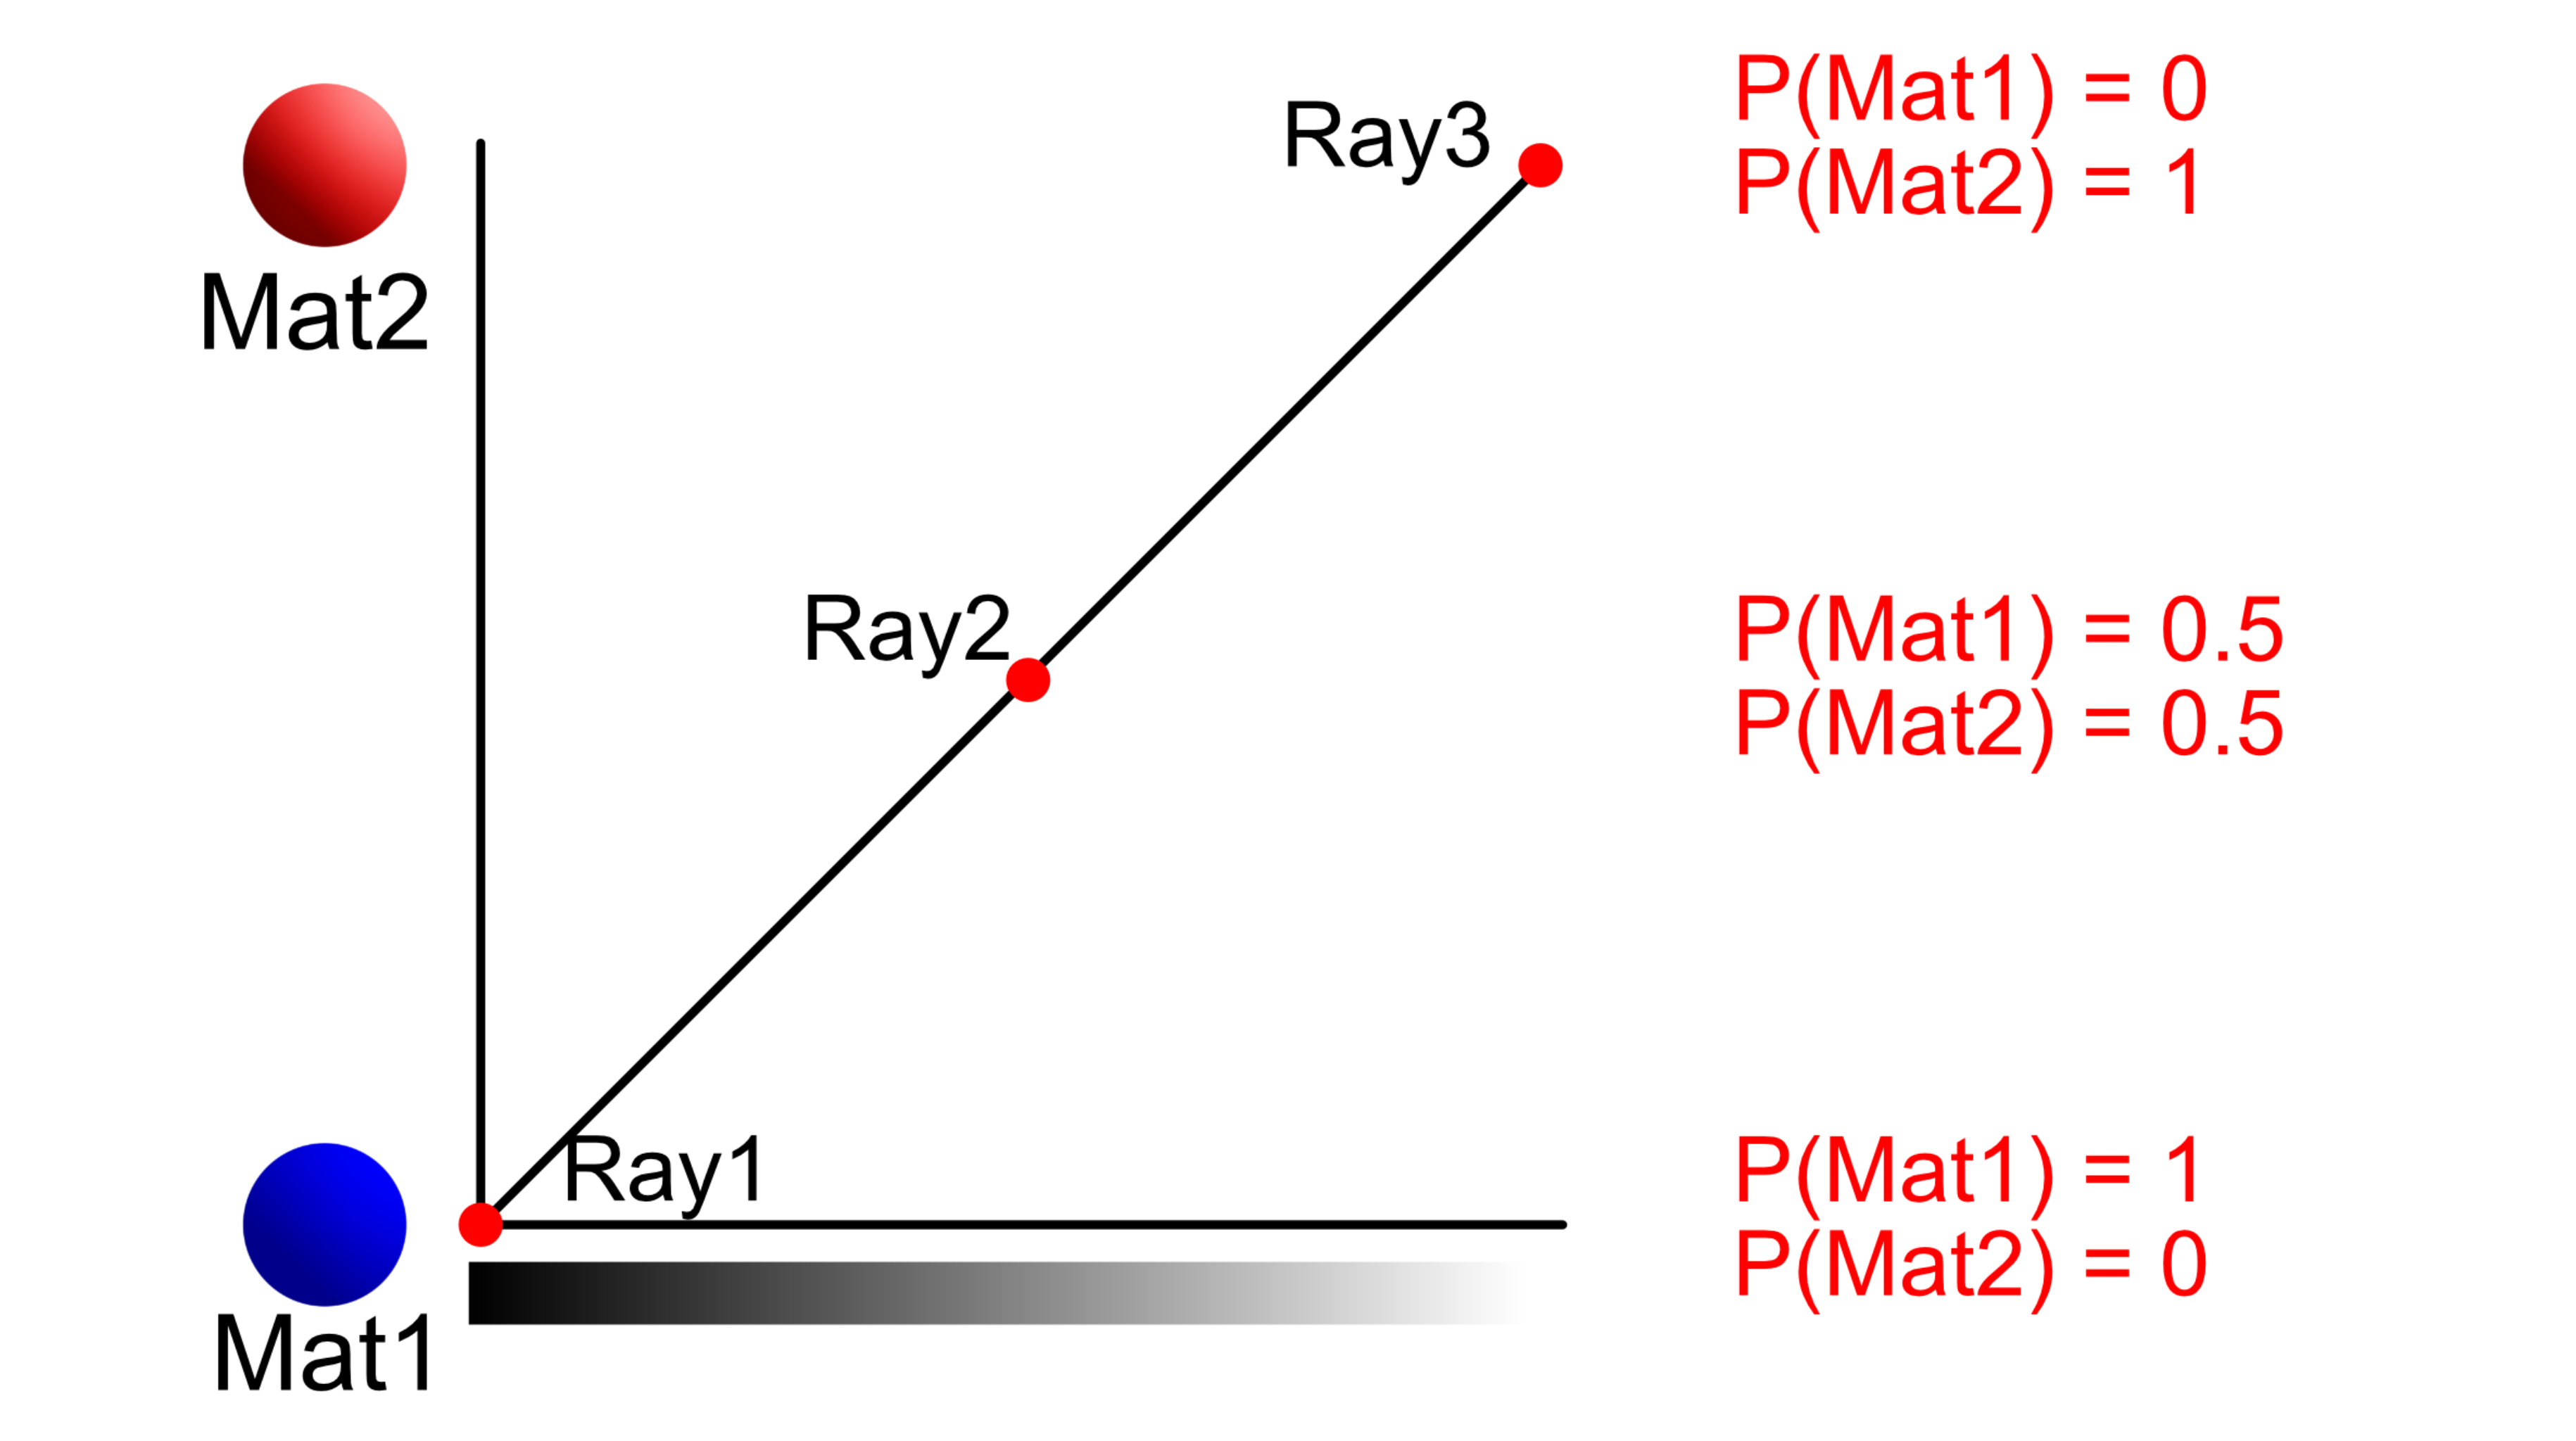
\includegraphics[width=.475\textwidth]{images/03cha_05_BxDFLayeringPdf.jpg} \\[6pt]
			(b) & (c) 
		\end{tabular}
			\caption{ \emph{BxDF layering} with two base materials.
				Figure (a) shows a shaded sphere with two BxDF materials blended together. They are combined using a linear gradient  from black to white as seen in figure (b), from the blue material \emph{Mat1} to the red material \emph{Mat2}. Rather than blending the output of both materials or the inputs, this method influences the probability density function of the render equation for the incoming rays. As shown in figure (c), the probability for the black masked area on the right side is a 100\% to hit the blue \emph{MAT1}. Going further to the right side of the object, this probability shifts more towards the red material \emph{MAT2}. The probability increases until it is finally a 100\% at the white masked areas.}
		\label{fig:BxDFLayering}
	\end{figure}

	\subsection{Illumination Lobe Based Layering}\label{sec:illuminationLobeLayering}

	Before going into detail about illumination lobe based layering, I want to talk briefly about lobes in the context of shading. A BxDF is composed of different lobes that define how the material interacts with light. Figure \ref{fig:lobes} illustrates this fact. \emph{Pixars} \emph{PxrSurface} is an \emph{Uber Shader} dedicated to replicate all kinds of different materials. To make this possible, the material properties are described by ten different lobes (e.g., diffuse, three specular, glass, subsurface etc.). For the basic BxDF shading these lobes are mixed linearly together. The principle behind illumination lobe based layering is to stack different base materials that use a different set of illumination lobes. These lobes are than stacked onto one another by also replicating the physical thickness of a material layer.   
	
	All the previously explained methods are able to yield astonishing results but fail to simulate the light propagation in a physically plausible way. The illumination lobe base layering is the only approach presented in this work that aims to imitate the real world behavior of different, distinctive layers stacked on one another. Wenzel Jakob provides some examples for surface properties that are not possible to recreate with the traditional BxDF shading models. Some of these examples are: ceramic covered by glaze, colored car paint with an additional layer of clear coat and biological layered materials like skin or leafs \cite[p.\,1]{jakob2015layerlab}. He further explains the challenging task of recreating this complex real world materials in following paragraph from \cite[p.\,1]{jakob2015layerlab}:
	
	%from the article \emph{layerlab: A computational toolbox for layered materials} \cite[p.\,1]{jakob2015layerlab} are: glaze over ceramic, wall, paint over primer, colored car paint with a clear coat, enamel on gold and silver jewelry, and layered biological structures such as leaves or skin``.
	
	\begin{itquote}
		Simulating these types of layered materials in renderings is surprisingly difficult: when a quantum	of light enters the top layer, it can undergo a complex sequence of scattering events within individual layers and at layer boundaries; finally, the light is either absorbed or able to leave the material. The	details of this intermediate scattering process are important, since they determine both the intensity and distribution of scattered light. [\ldots] Even the simplest nontrivial system, of a single medium bounded by a smooth interface, is only roughly approximated by standard BRDF models [\ldots].
	\end{itquote} 
	
	Recreating this complex effect has been a subject of interest over the last years. A lot of solutions have been proposed and adopted to recreate a really specific case. \emph{Tencent} and \emph{Epic Games} have shown an astonishing result for a real-time skin shader using an additional glossy specular layers stacked over the base shader and an additional specular lobe underneath it in \cite{seymour2018StateOfUe}. Estevez et al. \cite[p.\,1]{estevez2017production} propose an efficient method to simulate the back scattering characteristics of fabrics by introducing an additional sheen specular lobe. The current methods used for real-time productions are limited to one specific kind of material, e.g., skin, fabric or coated paint. Therefore, a lot of research has been going on to create an illumination lobe based material layering system that works for arbitrary base materials and any number of layers.
	
	One attempt do do so was developed by Jakob et al. \cite{jakob2014comprehensive}. They developed a framework to compute layered materials for arbitrary isotropic and anisotropic layers with smooth or rough	boundaries of conductors and dielectrics. Their paper has been the starting point for a lot of ongoing research. Their layered material system has just recently been expanded by Zeltner et al. \cite{jakob2018labratory} to cover reflective, transmissive, anisotropic layers as well. The limitations of these approaches are their heavy reliance on precomputed and stored data. These methods do not support varying texture materials inputs as they rely on precomputed data. 
	
	Belcour has recently released a paper \cite{laurent2018efficient} containing a  real-time compatible new framework. This work targets a comparable visual quality to preview methods proposed by Jakob et al. \cite{jakob2014comprehensive} and Zeltner et al. \cite{jakob2018labratory}. In contrast to their work, Belcour's method, presented in \cite{laurent2018efficient}, does not rely as heavily on precomputed tabular data but relies rather on statistical analysis and decomposes ``light transport into a set of atomic operators that act on its directional statistics''. Finally, also this approach relies on stored data but with a much smaller footprint. The paper contains an implementation example for both offline and real-time rendering. Both share the same code for the greatest extent. The real-time implementation has some limitations (e.g., restricted to three base materials and two output lobes) regarding the increase of efficiency. Other limitations common to both renderer are: In cases with several glossy materials, the specular lobes of the output gets inaccurate, anisotropic and subsurface scattering is not implemented, only the GGX algorithm for the specular reflection is implemented and the approximation that light enters and exits the material at the same point is made. Belcour specifies which technical criteria a layered material approach has to fit to be suitable for production \cite[p.\,73]{laurent2018efficient}:     
	
	\begin{itquote}
		A key difficulty is to provide a realistic model that works with an arbitrary number of layers (possibly textured), accounts for multiple scattering, is energy conserving, requires little storage, has a short precomputation time, supports good importance sampling and is symmetric with respect to light transport evaluation (to be compatible with bidirectionnal rendering techniques). 
	\end{itquote}

	\begin{figure}
		\begin{tabular}{@{}cc@{}}
			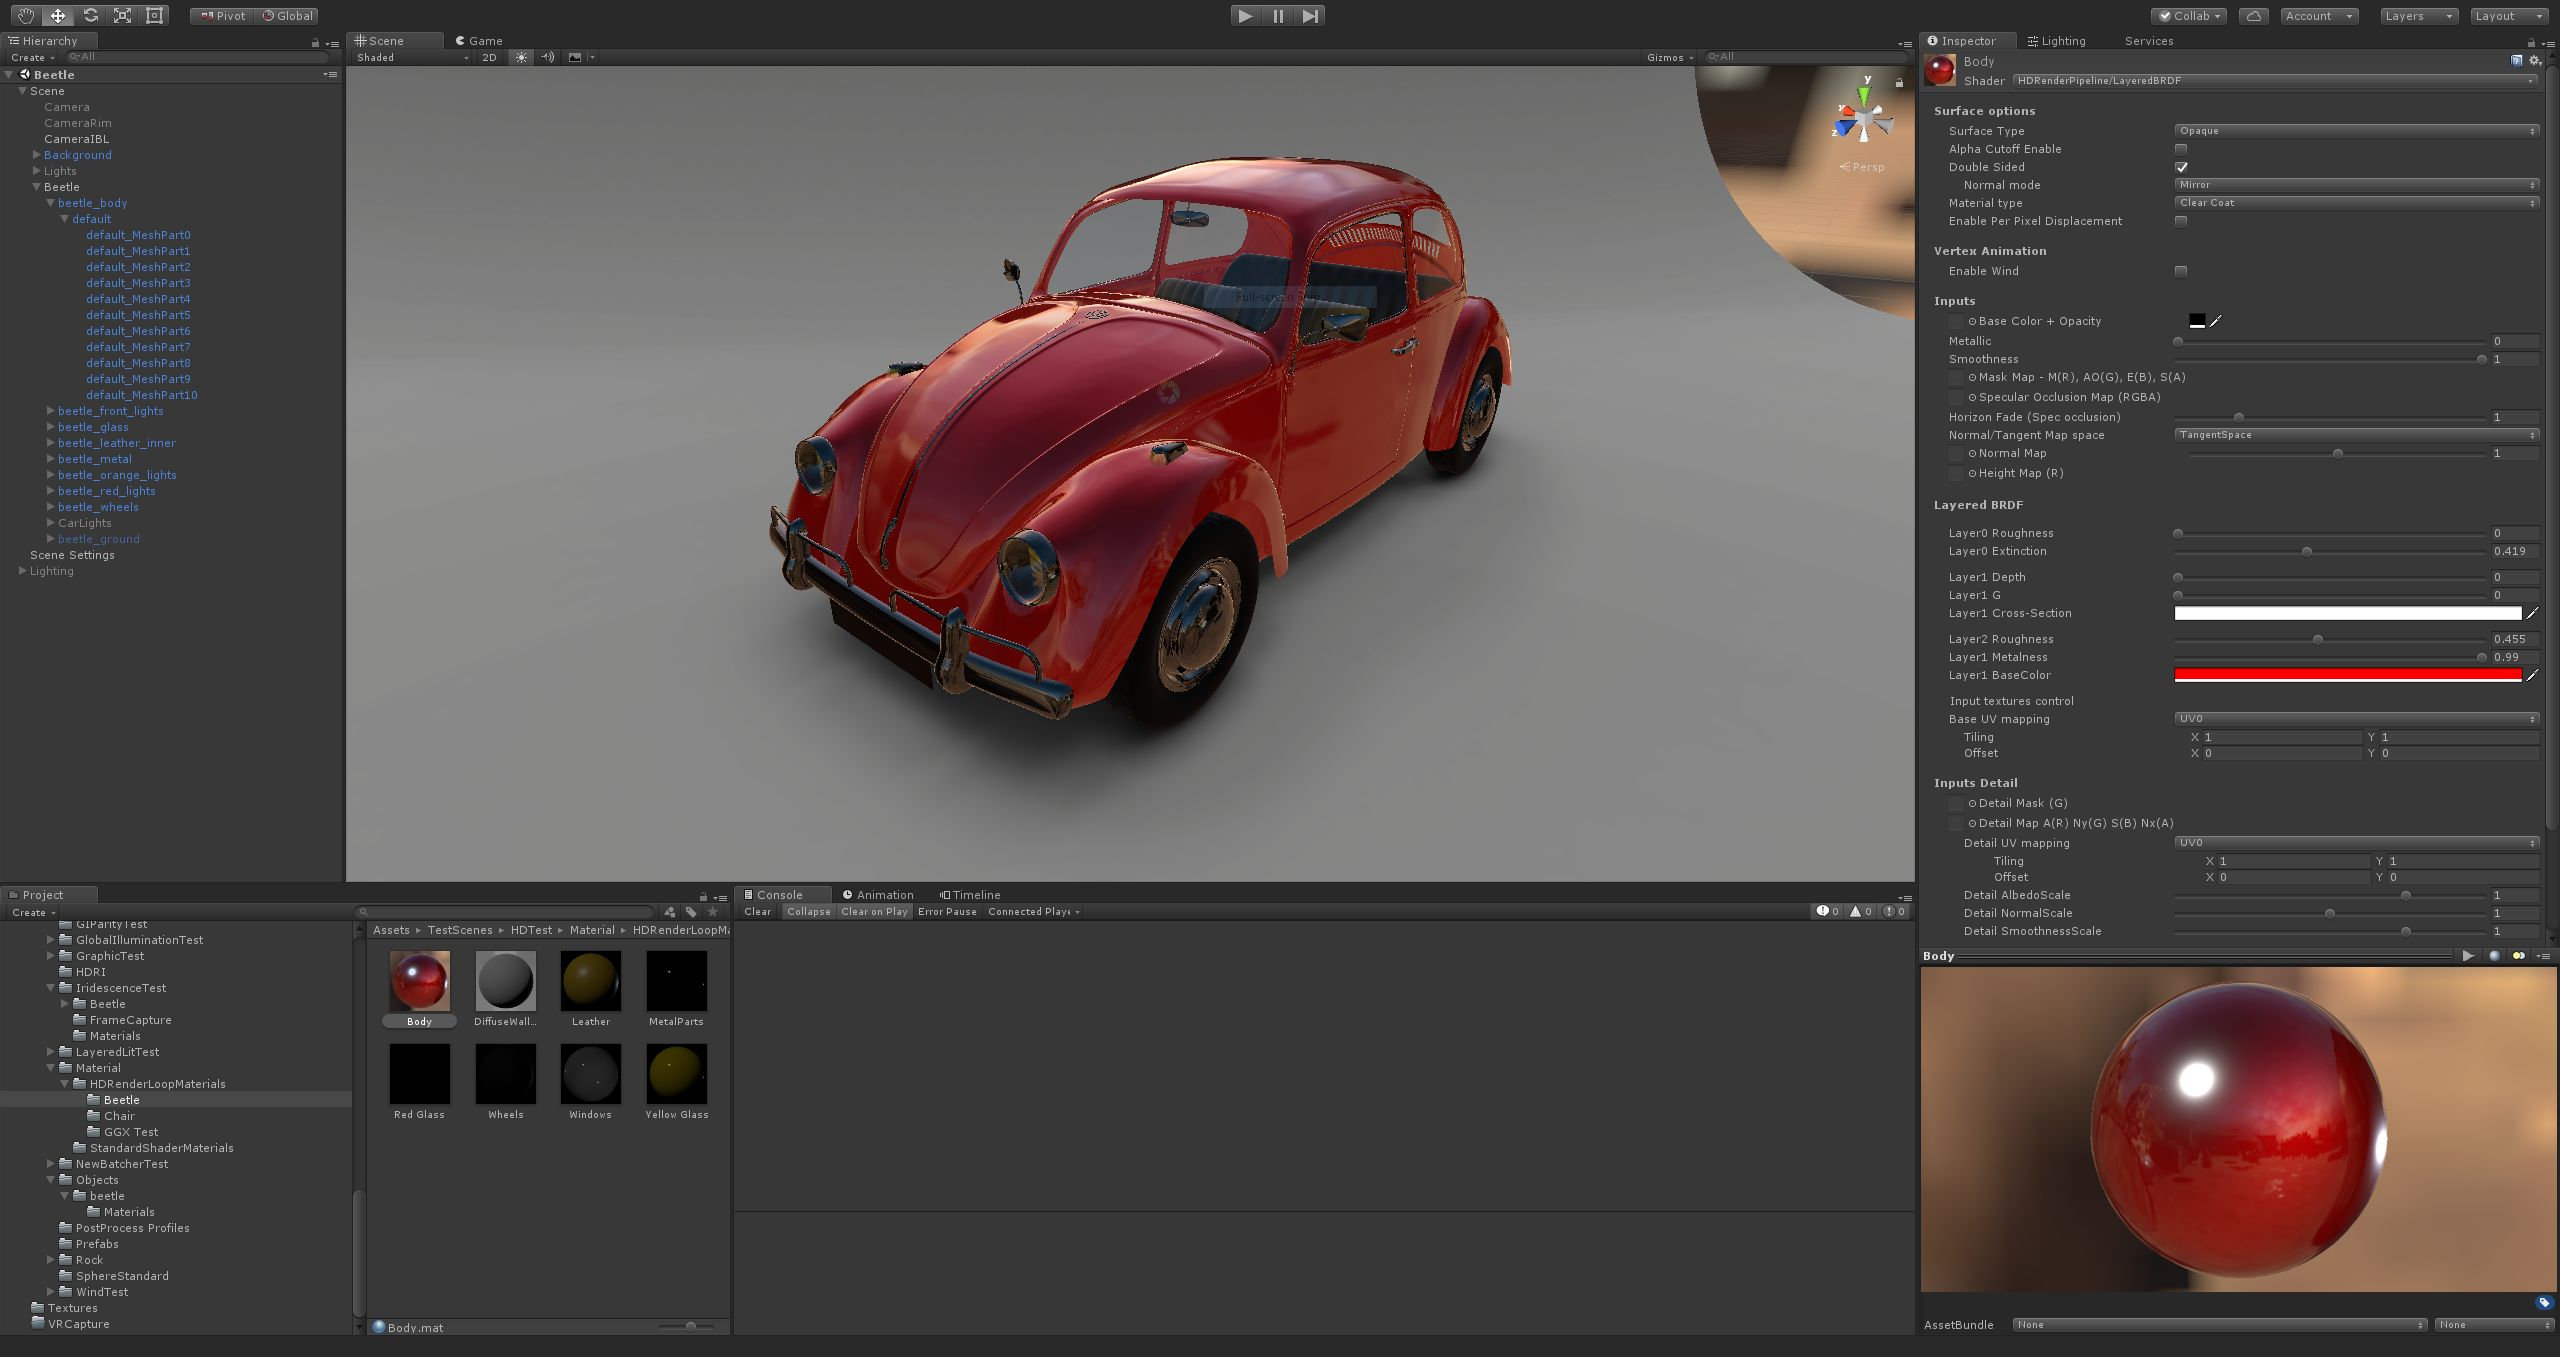
\includegraphics[width=0.475\textwidth]{images/03cha_06_raalTimeLobeBeatle.jpg} &		% JPEG file
			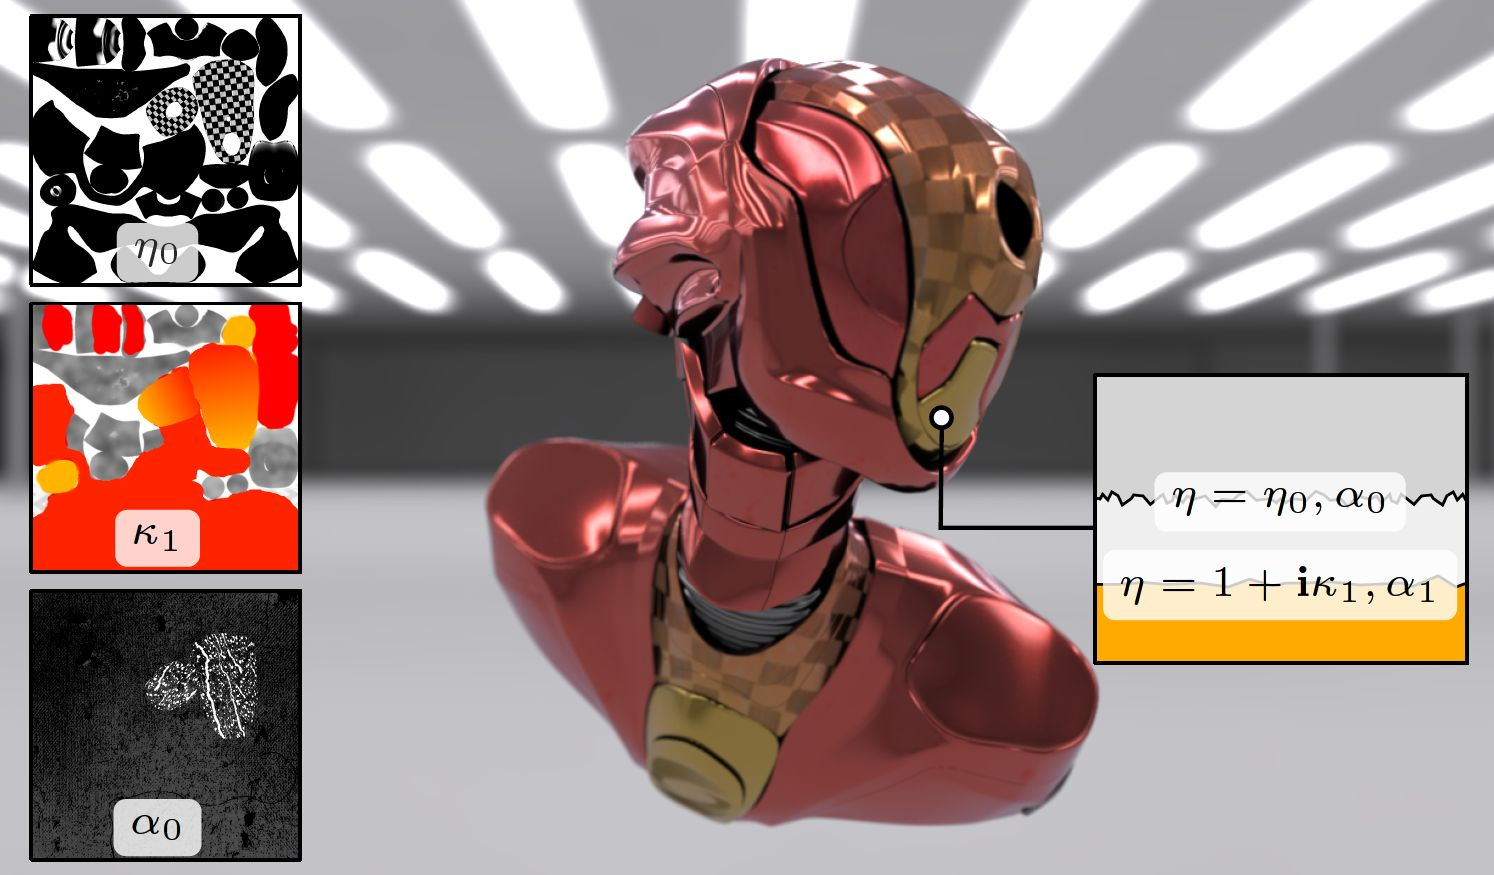
\includegraphics[width=0.475\textwidth]{images/03cha_06_robotOfflineLobeLayering.jpg} \\
			(a) & (b) 
		\end{tabular}
		\caption{Illumination Lobe Based Rendering in both a real-time (a) and offline renderer (b). Image source: \cite[p.\,73:11]{laurent2018efficient}.}
		\label{fig:lobeBasedRealTime}
	\end{figure}

	
	\begin{figure}
		\centering
		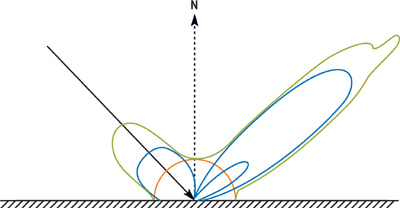
\includegraphics[width=0.5\textwidth]{images/03cha_07_IlluminationLobes.jpg}
		\caption[Color Layering]{
			A material composed of four different lobes. The orange line represents the diffuse component, the three blue lines are additional lobes (e.g., specular lobes) and the green line shows all the lobes combined that into the BRDF. This is a visible representation of the reflectance at each and every point for every possible incoming and outgoing angle. Image source: \cite{fernando2004gems}.}
		\label{fig:lobes}
	\end{figure}	
	


\section{Summary}

In this chapter, different methods of material layering were discussed. An important differentiation was made between material blending and material coating. In contrast to material blending, material coating is not used to blend different base materials but does rather simulate the complex scattering of light happening between multiple thin layers. A further categorization of material layering methods was made based on an article by Davide Pesare \cite{pesare2017material}; \emph{color layering}, \emph{pattern layering}, \emph{BxDF layering} and \emph{illumination lobe based layering}.  
Table \ref{table:materialLayeringSummary} summarizes the key differences of these methods. Color layering and illumination lobe based layering are not officially implemented in any of the game engines. Color layering can be achieved by using custom render passes. This is expensive as the material needs to be rendered several time. Therefore, it is not used for material layering in real-time applications. Belcour proposes a method to implement a simplified illumination lobe based layering system into a real-time engine in \cite{laurent2018efficient}.

\begin{table}
	\caption{Overview of the material layering methods.}
	\label{table:materialLayeringSummary}
	\centering
	\begin{longtable}{|p{2.5cm}|p{0.75cm}|p{0.75cm}|p{9cm}|}
		\hline
		\small
		Material Layering Method                          & \rotatebox[origin=c]{90}{Material Coating} & \rotatebox[origin=c]{90}{Game Engine Support} & Description                                                                                                                                                                                                                                                                                                                                                  \\ \hline
		Color layering                  & -       & $\sim$                         & Each material is rendered independently and stored in an RGBA layer. The render layers are blended together by using the alpha channels. There are some advanced techniques to account for complex shading techniques like displacement blending.                                                                                                                                                                                  \\ \hline
		Pattern layering                & -       & X                         & 
		The idea behind pattern layering is to rather blend the material inputs then their outputs. The different inputs from one base material like base color, roughness and metallic get blended with the inputs of another base material and combined into one material by the shader. Finally, these blended parameters define how the material affects the corresponding rendering passes. \\ \hline
		BxDF layering                   & -       & -                         & BxDF layering does neither blend the inputs nor outputs of the base materials but rather influences the probability density function within a ray tracer. This means it influences the probability with which an incoming ray hits a certain material. The materials and the blending process are independent from one another.                                                                                                                \\ \hline
		Illumination lobe base layering & X       & $\sim$                     & Illumination lobe based layering is the only method that accounts for the complex process of light passing through different layers and being manipulated by them. It imitates the complex scattering and modulation of light when passing through different layers with a thickness and different physical properties. \\ \hline
	\end{longtable}
\end{table}

